\documentclass[11pt]{article}
\usepackage[a4paper,margin=24mm]{geometry}
\usepackage{amsmath,amssymb,booktabs,graphicx}
\graphicspath{{../../figures/paper/echo_dip_theory/}}
\usepackage[section]{placeins}
\usepackage[colorlinks=true,urlcolor=blue,linkcolor=blue]{hyperref}
\newcommand{\Pe}{P_e}
\newcommand{\Om}{\Omega}
\title{Echo-pulse spectroscopy: the central dip and its linewidth}
\author{Audited theoretical note with numerical comparisons}
\date{14 October 2026}
\begin{document}
\maketitle

\begin{abstract}
A symmetric drive with a midpoint sign reversal has exactly zero resonant
excitation in an ideal two-level system. We derive its near-resonant curvature
without expanding in drive strength, and obtain a closed expression for a
finite root-Lorentzian pulse. Separately, an adiabatic treatment of the two
halves predicts a Lorentzian depletion with cyclic-frequency FWHM
$\Gamma_f\simeq\Om_0c/\pi=2c f_{\rm Rabi}$ when truncation dominates.
This is a regime-dependent linewidth, not a universal echo linewidth.
Endpoint smoothing, dissipation, and multilevel effects are discussed below.
\end{abstract}

\noindent\textbf{Audit outcome.} The exact resonant cancellation and curvature
survive independent numerical checks. The adiabatic line shape is a useful
strong-drive approximation, but its half-height width must not be confused
with a half-depth width relative to nonunit shoulders. Two qualifications
have been tightened: the approximation for $C$ additionally requires
$ac\ll1$, and the polynomial $1/7$ exponent is an asymptotic edge argument,
not a general fit to the working waveform. Figures~\ref{fig:mechanism}--\ref{fig:dissipation}
plot the equations against new simulations. No parameters are fitted in the
root-Lorentzian line-shape comparison.

\section{Model and the exact resonant cancellation}
Use the repository convention $\Delta=\omega_d-\omega_{01}$ and define
$\sigma_z=|g\rangle\langle g|-|e\rangle\langle e|$. Dropping an identity
term, the rotating-wave Hamiltonian is
\begin{equation}
 H(t)/\hbar=\tfrac12[\Delta\sigma_z+\Om_E(t)\sigma_x],\qquad
 \Om_E(t)=\Om_0 g(t)s(t),\qquad -h\le t\le h,\quad h=L/2.
 \label{eq:model}
\end{equation}
Here $g(-t)=g(t)$ is real and $s(-t)=-s(t)$; the abrupt echo has
$s(t)=+1$ before the midpoint and $-1$ after it. All $\Om$ and $\Delta$
are angular frequencies. The initial state is $|g\rangle$ and the observable
is the population immediately after the pulse.

At $\Delta=0$ all Hamiltonians commute. Consequently,
\begin{equation}
 U_0(h,-h)=\exp\left[-\frac{i\sigma_x}{2}
 \int_{-h}^{h}\Om_E(t)\,dt\right]=\mathbb I,
 \qquad \boxed{\Pe(0)=0.}
 \label{eq:zero}
\end{equation}
The result is independent of amplitude and pulse area. A common multiplicative
amplitude error preserves the zero. Unequal half areas do not: if their signed
sum is $\epsilon$, then $\Pe(0)=\sin^2(\epsilon/2)\simeq\epsilon^2/4$.
An odd, smooth, real sign transition also preserves Eq.~\eqref{eq:zero}.
A second drive quadrature or a time-dependent frequency shift generally
invalidates this commuting-Hamiltonian argument.

\subsection{An exact propagator identity for the echo}
There is a useful independent way to check the entire coherent spectrum.
For a real symmetric Hamiltonian, reversing its time order transposes its
propagator, as used for symmetric ordinary pulses in Ref.~\cite{smooth2024}.
For the echo, $H(t)=\sigma_z H(-t)\sigma_z$. If the first-half propagator is
\begin{equation}
 U_1=\begin{pmatrix}A&B\\-B^*&A^*\end{pmatrix},\qquad
 |A|^2+|B|^2=1,
\end{equation}
then
\begin{equation}
 U_2=\sigma_z U_1^{\mathsf T}\sigma_z,\qquad
 \boxed{\Pe=4[\operatorname{Re}(AB)]^2.}
 \label{eq:half-identity}
\end{equation}
This identity is exact for an odd real waveform, including the smoothed
polynomial pulse; no adiabatic assumption is made. It provides a numerical
cross-check using a separately propagated half pulse. The phase reversal
is the rotary-echo operation, whose optical realization and Bloch-equation
description are discussed in Ref.~\cite{rotary1980}.

\section{An exact small-detuning result, including strong drives}
Define the accumulated signed rotation
\begin{equation}
 \theta(t)=\int_{-h}^{t}\Om_E(t')\,dt',\qquad
 U_0(t)=e^{-i\theta(t)\sigma_x/2}.
\end{equation}
Transforming away this drive gives
\begin{equation}
 H_I(t)/\hbar=\frac{\Delta}{2}
 [\sigma_z\cos\theta(t)+\sigma_y\sin\theta(t)].
\end{equation}
Introduce two quantities with units of time,
\begin{equation}
 S=\int_{-h}^{h}\sin\theta(t)\,dt,\qquad
 C=\int_{-h}^{h}\cos\theta(t)\,dt.
 \label{eq:SC}
\end{equation}
The first Dyson term is
$U_I=\mathbb I-i\Delta(C\sigma_z+S\sigma_y)/2+O(\Delta^2)$.
Only $\sigma_y$ transfers population, so
\begin{equation}
 \boxed{\Pe(\Delta)=\frac{\Delta^2 S^2}{4}+O(\Delta^4),\qquad
 \Pe''(0)=S^2/2.}
 \label{eq:curvature}
\end{equation}
Population is even in detuning for this real, coherent two-level model;
hence no cubic term occurs. This curvature is exact at any drive amplitude.
It is a local expansion, conservatively controlled by $|\Delta|L\ll1$,
and does not determine the off-resonant shoulder height.

\subsection{Closed form for the hard-cutoff root-Lorentzian}
Take
\begin{equation}
 g(t)=\frac{1}{\sqrt{1+(t/\tau)^2}},\quad
 c=g(h),\quad
 \tau=\frac{hc}{\sqrt{1-c^2}},\quad
 u_c=\operatorname{asinh}(h/\tau)=\operatorname{arcosh}(1/c),\quad
 a=\Om_0\tau.
\end{equation}
For the abrupt echo,
$\theta(t)=a[u_c-\operatorname{asinh}(|t|/\tau)]$.
Substitution $|t|=\tau\sinh u$ into Eq.~\eqref{eq:SC} yields
\begin{align}
 S&=2\tau\int_0^{u_c}\cosh u\sin[a(u_c-u)]\,du
   =\boxed{\frac{2\tau a}{1+a^2}
   [\cosh u_c-\cos(a u_c)]},\label{eq:Sroot}\\
 C&=\frac{2\tau}{1+a^2}[\sinh u_c+a\sin(a u_c)].
\end{align}
For $c\ll1$, the relative oscillatory correction in $S$ is small. The
corresponding simplification for $C$ additionally needs $ac\ll1$:
\begin{equation}
 S\simeq\frac{La}{1+a^2},\qquad C\simeq\frac{L}{1+a^2},\qquad
 \Pe(\Delta)\simeq\frac{(\Delta L)^2}{4}
                   \frac{a^2}{(1+a^2)^2}.
 \label{eq:local-simple}
\end{equation}
Indeed, the relative omitted term in $C$ is
$a\sin(a u_c)/\sinh u_c\simeq ac\sin(a u_c)$ and is not uniformly small
at arbitrarily large $a$. The approximation for $S$ and the curvature do
not need this additional condition.
At fixed $L,c$, curvature initially increases with drive, is largest near
$a=1$, and decreases at large $a$. This predicts a change in the local
dip sharpness; it does not by itself locate a minimum in FWHM, since dip
depth can change too. For $a\gg1$, $S\simeq L/a\simeq2/(\Om_0c)$.

\begin{figure}[htbp]
\centering
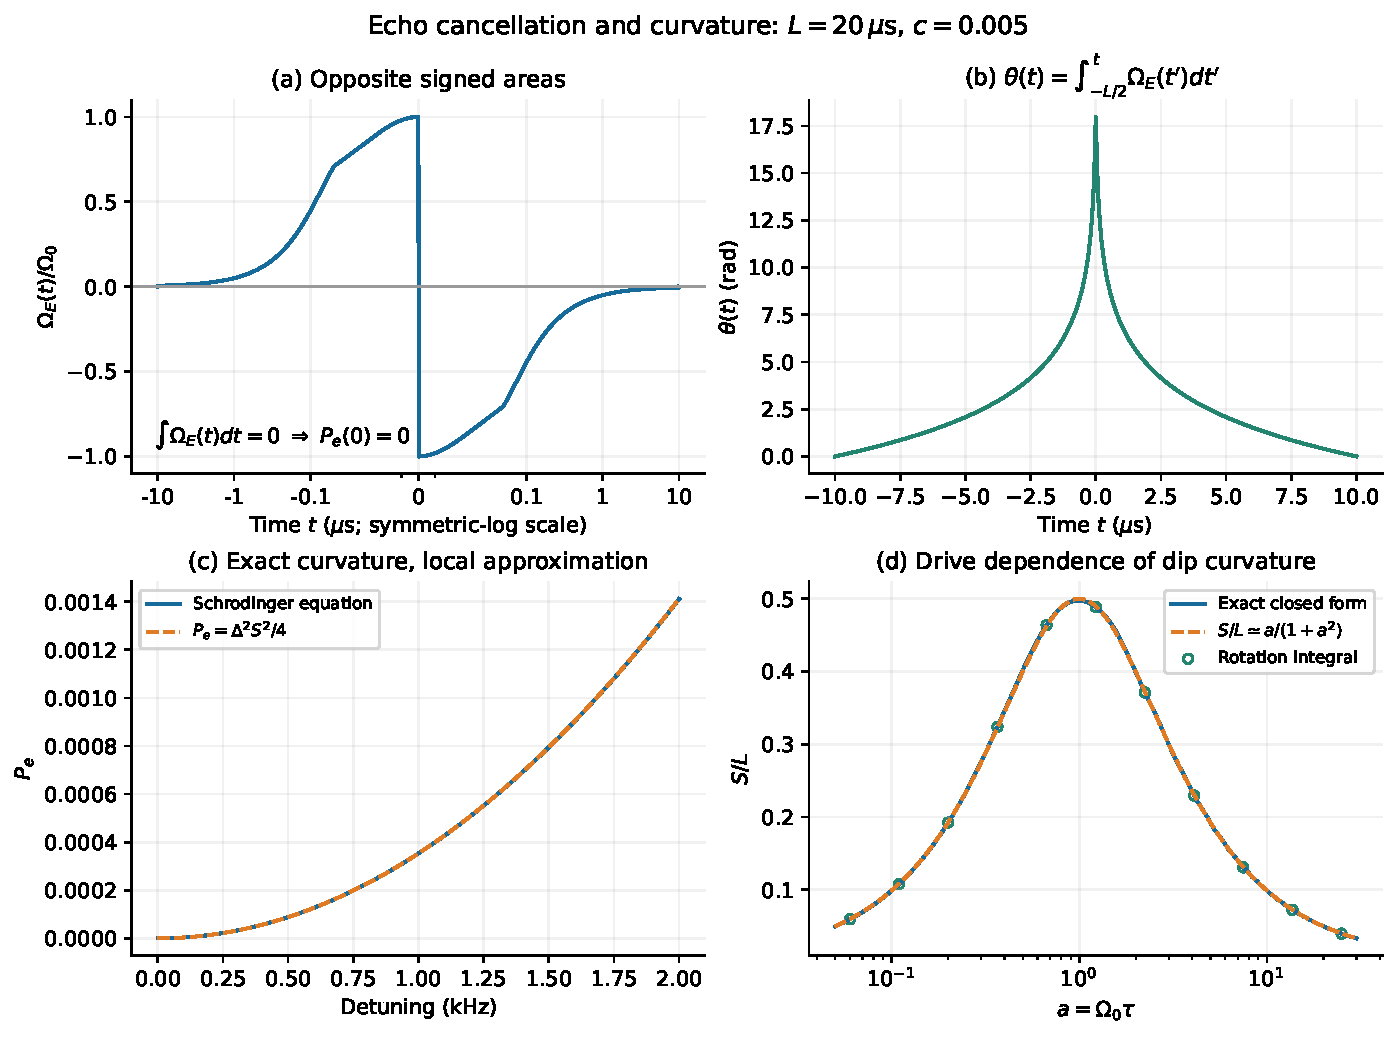
\includegraphics[width=\textwidth]{01_mechanism_curvature.pdf}
\caption{Equations~\eqref{eq:zero}, \eqref{eq:curvature}, and
\eqref{eq:Sroot} visualized. Panels (a)--(c) use $a=3$, $L=20\,\mu$s,
and $c=0.005$. The signed area cancels while the accumulated rotation
returns to zero. The quadratic line shape agrees locally with the full
Schr\"odinger dynamics. Panel (d) compares the exact closed-form $S$ with
direct integration of $\theta(t)$ and its small-cutoff approximation.
The maximum at $a\simeq1$ is a maximum of curvature, not an independently
established optimum in FWHM or sensitivity.}
\label{fig:mechanism}
\end{figure}

\section{A line shape and FWHM from adiabatic evolution of each half}
The preceding result requires no adiabatic assumption. To obtain an entire
central line shape, now assume an abrupt midpoint inversion and adiabatic
evolution \emph{inside each half}. Treat both outer jumps and the midpoint
jump explicitly; they are not assumed adiabatic.

For positive detuning define
\begin{equation}
 q(t)=\sqrt{\Delta^2+\Om_0^2g(t)^2},\quad
 \vartheta(t)=\arctan[\Om_0g(t)/\Delta],\quad
 \Phi=\int_{-h}^0q(t)\,dt.
\end{equation}
Write $R(\vartheta)=e^{-i\vartheta\sigma_y/2}$,
$Z(\Phi)=e^{-i\Phi\sigma_z/2}$, and let $\vartheta_e,\vartheta_0$
be the edge and center mixing angles. With $\Om_e=\Om_0c$,
\begin{align}
 U_1&\simeq R(\vartheta_0)Z(\Phi)R(-\vartheta_e),\\
 U_2&\simeq R(-\vartheta_e)Z(\Phi)R(\vartheta_0),\\
 U_E&\simeq R(-\vartheta_e)Z(\Phi)R(2\vartheta_0)
                       Z(\Phi)R(-\vartheta_e).
\end{align}
Multiplying these matrices gives
\begin{equation}
 \boxed{\Pe^{\rm ad}(\Delta)=
 \frac{\Delta^2[\Om_0-\Om_e\cos\Phi]^2}
 {(\Delta^2+\Om_e^2)(\Delta^2+\Om_0^2)}.}
 \label{eq:adiabatic-full}
\end{equation}
The population extends evenly to negative detuning. For the root-Lorentzian,
the phase is a single smooth quadrature,
\begin{equation}
 \Phi=a\int_0^{u_c}
 \sqrt{1+(\Delta/\Om_0)^2\cosh^2u}\,du.
\end{equation}
As a check, setting $c=1$ and using a constant half-pulse amplitude reduces
Eq.~\eqref{eq:adiabatic-full} to the exact square-echo result
\begin{equation}
 \Pe^{\rm square}=
 \frac{4\Delta^2\Om_0^2}{(\Delta^2+\Om_0^2)^2}
 \sin^4\left[\frac{L}{4}\sqrt{\Delta^2+\Om_0^2}\right].
\end{equation}

For $c\ll1$ and $|\Delta|\ll\Om_0$, Eq.~\eqref{eq:adiabatic-full}
simplifies to
\begin{equation}
 \boxed{\Pe(\Delta)\simeq\frac{\Delta^2}{\Delta^2+(\Om_0c)^2}
 =1-\frac{1}{1+[\Delta/(\Om_0c)]^2}.}
 \label{eq:lorentzian}
\end{equation}
Thus the \emph{depletion} is Lorentzian, relative to a local excited-state
shoulder near unity. The shoulder is local: the finite pulse eventually
ceases to excite the qubit at very large detuning. Half-depth crossings are
$\Delta_\pm=\pm\Om_0c$, giving
\begin{equation}
 \boxed{\Gamma_\omega\simeq2\Om_0c,\qquad
 \Gamma_f=\Gamma_\omega/(2\pi)\simeq\frac{\Om_0c}{\pi}
 =2c f_{\rm Rabi}.}
 \label{eq:width}
\end{equation}
For example, $c=0.005$ and $f_{\rm Rabi}=10\,\mathrm{MHz}$ give a
cutoff-dominated estimate of $100\,\mathrm{kHz}$.

The physical origin is especially clear when $\vartheta_0\simeq\pi/2$:
$Z(\Phi)R(\pi)Z(\Phi)=R(\pi)$ cancels the dynamical phases, and
$U_E\simeq R(\pi-2\vartheta_e)$. The remaining response is set by the
mixing angle at the \emph{outer edge}. A residual endpoint drive therefore
produces cutoff broadening despite the exact resonant zero.

\subsection{When is this approximation justified?}
The local adiabatic parameter is
\begin{equation}
 \eta(t)=\frac{|\dot\vartheta|}{2q}
 =\frac{|\Delta\dot\Om|}{2(\Delta^2+\Om^2)^{3/2}}\ll1.
\end{equation}
In a root-Lorentzian wing $\Om\simeq a/|t|$, putting
$r=\Om/|\Delta|$ gives
$\eta\simeq r^2/[2a(1+r^2)^{3/2}]$, bounded by
$1/(3\sqrt3a)$. Thus $a\gg1$ is a useful sufficient wing criterion,
in addition to $c\ll1$ and a fast midpoint jump.
The exact curvature in Eq.~\eqref{eq:Sroot} tends to
$\Pe\simeq\Delta^2/(\Om_0c)^2$ in the same regime, independently checking
the Lorentzian result. At $a\lesssim1$, its curvature differs by the factor
$a^4/(1+a^2)^2$ to leading order in small $c$; using Eq.~\eqref{eq:width}
there is unjustified.

\begin{figure}[htbp]
\centering
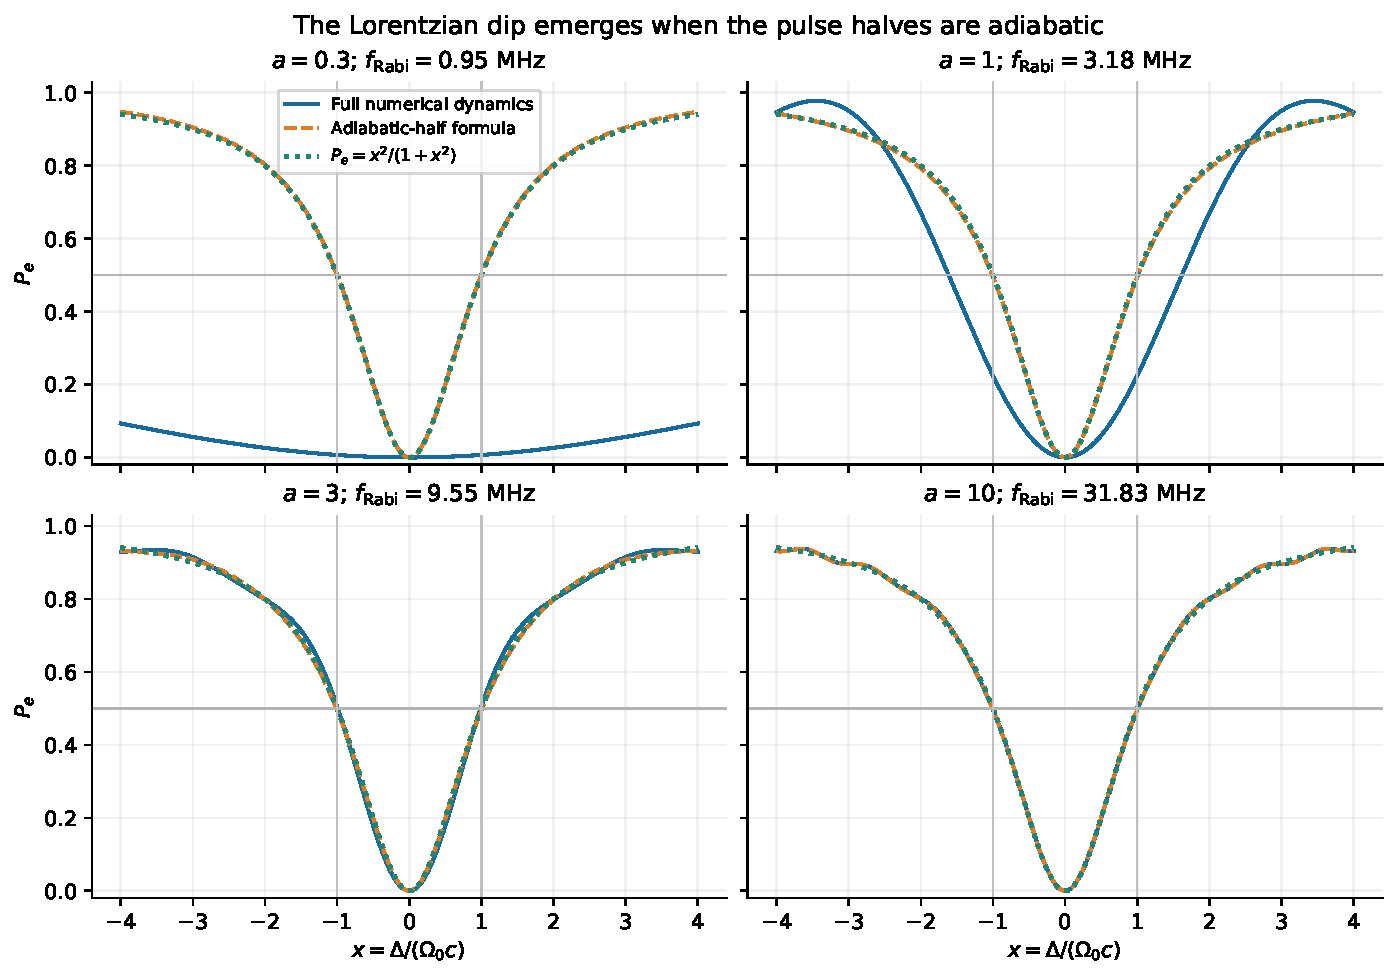
\includegraphics[width=\textwidth]{02_lineshapes.pdf}
\caption{Full coherent spectra compared with the adiabatic-half expression,
Eq.~\eqref{eq:adiabatic-full}, and the simplified Lorentzian depletion,
Eq.~\eqref{eq:lorentzian}. All panels use $L=20\,\mu$s and $c=0.005$;
the approximations have no fitted amplitude, center, or width. Vertical
lines at $x=\pm1$ mark the predicted half-height locations. The marked
failure at $a=0.3$ and the visible discrepancy at $a=1$ establish the
importance of the adiabatic assumption. All curves are ideal two-level
predictions, not transmon or experimental data.}
\label{fig:lineshapes}
\end{figure}

\section{What a local expansion can and cannot say about FWHM}
For a symmetric dip with locally flat shoulder $B$, center $P_0$, and depth
$D=B-P_0>0$, half depth means $\Pe=P_0+D/2$. If one extrapolates the
parabola in Eq.~\eqref{eq:curvature}, its width estimate is
\begin{equation}
 \Gamma_f^{\rm parabola}\simeq\frac{\sqrt{2D}}{\pi|S|}.
\end{equation}
If one instead assumes a Lorentzian depletion and matches its curvature,
\begin{equation}
 \Pe(\Delta)=P_0+D\frac{\Delta^2}{\Delta^2+\gamma^2},\qquad
 \gamma=\frac{2\sqrt D}{|S|},\qquad
 \Gamma_f^{\rm Lorentzian}\simeq\frac{2\sqrt D}{\pi|S|}.
\end{equation}
These differ by $\sqrt2$ despite identical curvature. Therefore an accurate
local expansion alone does not establish a FWHM. The Lorentzian is physically
justified in the regime of Eq.~\eqref{eq:lorentzian}; elsewhere the shoulder
and crossings must be determined from the full spectrum. In particular,
inserting a measured $D<1$ into a coherent formula does not account for
decoherence-induced changes of curvature.

In Fig.~\ref{fig:widths} we explicitly separate two numerical observables.
The first, $W_{0.5}$, is twice the nearest positive $\Pe=0.5$ crossing,
converted to cyclic frequency. The second uses half the depth relative to
the first local maximum on either side, accepting a maximum only when its
prominence exceeds 0.001 in population. Small coherent ripples can move this
first maximum; consequently this second prescription is illustrative, not
a universal background estimator. Neither uses a fitted Lorentzian.

\begin{figure}[htbp]
\centering
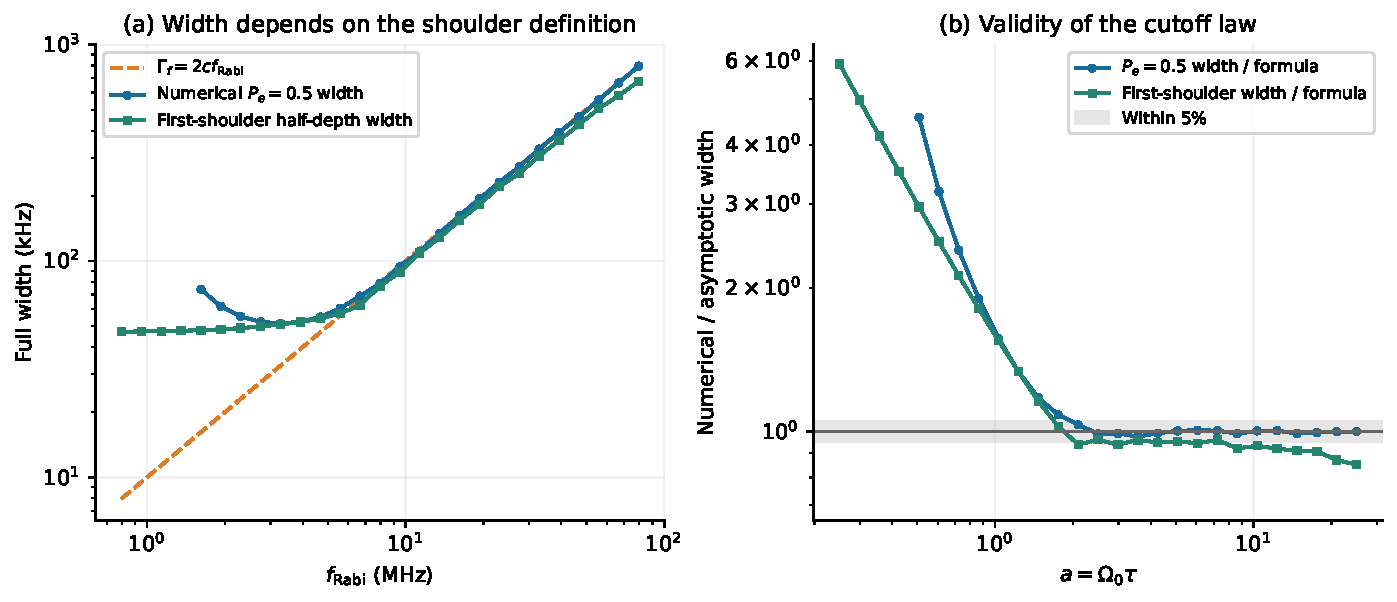
\includegraphics[width=\textwidth]{03_linewidth.pdf}
\caption{Width audit for $L=20\,\mu$s, $c=0.005$ and 27 values of
$a$ from 0.25 to 25. The cutoff law agrees with $W_{0.5}$ to within 2.52\%
for the tested $a\ge3$ points. The first-maximum half-depth width is
different because the shoulder is not identically one. At weak drive it
can remain defined even when $W_{0.5}$ does not exist because the entire
first excitation lobe lies below 0.5. Missing crossings are omitted.
The shaded band in (b) indicates a 5\% relative difference.}
\label{fig:widths}
\end{figure}

\section{Why the polynomial edge correction can reduce broadening}
For the project's cutoff-subtracted polynomial envelope,
\begin{equation}
 g_p(t)=\frac{[1+(t/\tau)^2]^{-1/2}-c}{1-c}
         [1-(t/h)^2]^p,\qquad |t|<h,
\end{equation}
the endpoint drive vanishes. One cannot simply set $\Om_e=0$ in
Eq.~\eqref{eq:lorentzian} and infer zero width: the edge dynamics cease to
be adiabatic near resonance.

Let $s=h-|t|\ll h$ be distance from an endpoint. For $0<c<1$,
\begin{equation}
 \Om(t)\simeq b s^m,\qquad
 m=p+1,\qquad b=\frac{\Om_0c(1+c)2^p}{h^{p+1}}.
\end{equation}
Rescaling time by $b^{-1/(m+1)}$ makes the local edge Schr\"odinger
equation depend on detuning through $\Delta/b^{1/(m+1)}$. Equivalently,
evaluating $\eta$ where $\Om\sim|\Delta|$ gives
$\eta\sim b^{1/m}|\Delta|^{-(m+1)/m}$, up to a factor depending on $m$.
Hence the characteristic nonadiabatic edge scale is
\begin{equation}
 \Delta_{\rm edge}\sim b^{1/(m+1)},\qquad
 \Gamma_f\sim\frac{K_p}{2\pi}
 \left[\frac{\Om_0c(1+c)2^p}{h^{p+1}}\right]^{1/(p+2)}.
 \label{eq:poly}
\end{equation}
Here $K_p$ is an undetermined dimensionless coefficient for a chosen
linewidth definition and edge-dominated regime. This is a candidate
\emph{scaling}, not a derived full echo line shape or a fitted result.
For $p=5$, it suggests a much weaker amplitude dependence,
$\Gamma_f\propto\Om_0^{1/7}$, than the hard-cutoff law
$\Gamma_f\propto\Om_0$. It requires the edge-interaction region to be
small relative to $h$, adiabatic interior evolution, and a sufficiently
fast midpoint inversion. It does not establish that existing finite-range
simulation scans have reached that asymptotic regime.

The common 16 ns sine sign transition preserves Eq.~\eqref{eq:zero} at
zero DRAG, and the general integral Eq.~\eqref{eq:SC} still applies.
The abrupt-jump derivation instead requires the Hamiltonian rotation during
the transition to be small; $T_{\rm tr}\max(\Om_0,|\Delta|)\ll1$ is a
sufficient condition. At high amplitudes, 16 ns need not be a sudden jump.
DRAG adds a second quadrature and requires a separate dynamical calculation.

\subsection{Numerical test of the working polynomial shape}
Figure~\ref{fig:shaping} compares the hard cutoff with the implemented
cutoff-subtracted $p=5$ envelope. The real waveform agrees pointwise with
\texttt{PolynomialEchoPulse.drive} at zero DRAG; the common 16 ns transition
is not peak-renormalized. For these plots, linewidth means half depth
relative to the mean population at $0.4\le|\Delta/(2\pi)|\le0.5$ MHz.
This equals a linear-background fit on the two bands for these exactly
even spectra. It differs from both definitions in Fig.~\ref{fig:widths}.

At $L=30\,\mu$s, $c=0.001$ and a nominal Rabi frequency of 100 MHz, the
ideal two-level widths are 190.37 kHz (abrupt hard cutoff), 189.80 kHz
(16 ns hard cutoff), and 118.62 kHz (16 ns polynomial). These numbers
exclude the DRAG and transmon effects present in the project's full model.
The polynomial width is 98.88 kHz at 10 MHz and varies weakly over the scan.
Its numerical logarithmic slope spans approximately $-0.070$ to $0.174$;
the high-drive values are close to $1/7$, but the full scan is not one power
law. The dashed $1/7$ reference is anchored at the last point only; its
absolute prefactor has not been predicted.

More directly, the edge-interaction length implied by Eq.~\eqref{eq:poly} is
\begin{equation}
 \frac{\ell}{h}=\frac{b^{-1/(p+2)}}{h}
 =\left[\Om_0 h c(1+c)2^p\right]^{-1/(p+2)}.
\end{equation}
It ranges from 0.61 to 0.44 in this scan, rather than being much less than
one. Thus this comparison supports weaker broadening from edge smoothing,
but does not establish a controlled asymptotic $1/7$ law for the whole
operating range. The generic finite-edge exponent is consistent with the
ordinary-pulse result of Ref.~\cite{edges2013}; applying it to the echo
dip still requires the assumptions stated above.

\begin{figure}[htbp]
\centering
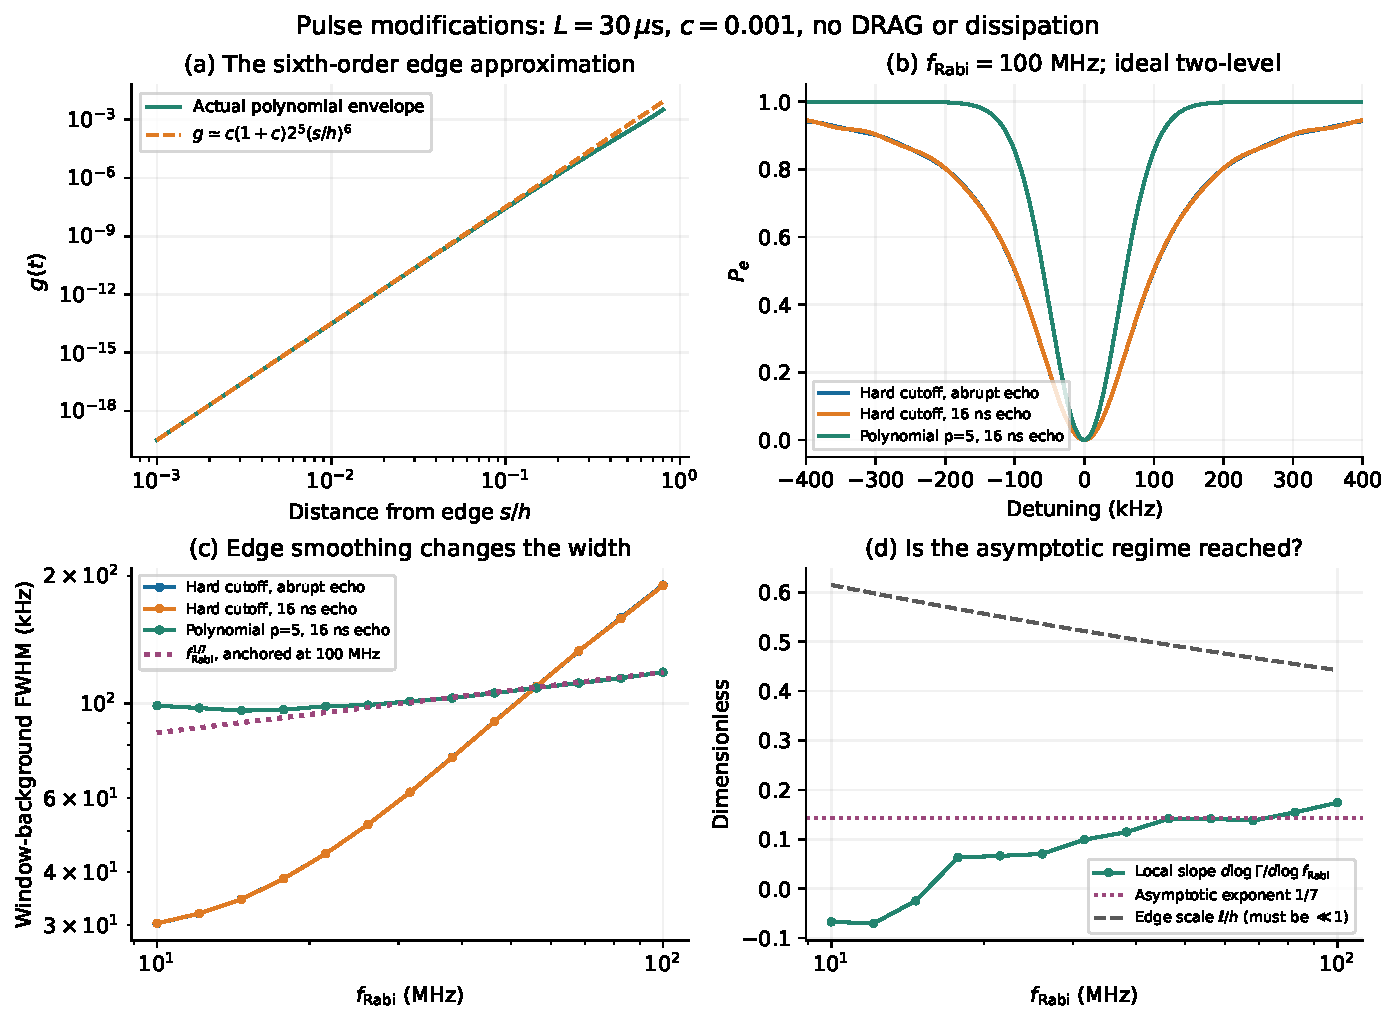
\includegraphics[width=\textwidth]{04_shaping.pdf}
\caption{Testing the polynomial-edge argument and midpoint smoothing.
(a) Actual envelope and its sixth-order expansion at the outer edge.
(b) Three full spectra at nominal $f_{\rm Rabi}=100$ MHz.
(c) Half-depth widths using the same $\pm(0.4$--$0.5)$ MHz background
bands for every curve. The $1/7$ line is normalized to the 100 MHz
polynomial point and is not a prediction of the absolute FWHM.
(d) Numerical local slope and the edge-interaction length. Their behavior
qualifies the domain of Eq.~\eqref{eq:poly}. All pulses have zero DRAG
and evolve without dissipation in an ideal two-level model.}
\label{fig:shaping}
\end{figure}

\section{Dip depth, dissipation, and the transmon}
For weak Markovian dissipation over the pulse, a first-order quantum-jump
expansion gives the on-resonance floor
\begin{equation}
 \boxed{\Pe(0)\simeq\int_{-h}^h
 \left[\frac{\sin^4[\theta(t)/2]}{T_1}
       +\frac{\sin^2\theta(t)}{2T_\phi}\right]dt.}
 \label{eq:floor}
\end{equation}
The jump operators are $|g\rangle\langle e|/\sqrt{T_1}$ and
$\sigma_z/\sqrt{2T_\phi}$. A relaxation jump at time $t$ has excitation
probability $\sin^2[\theta(t)/2]$ before the jump; the remaining reversed
drive excites the reset state with the same factor. A dephasing jump has
final transition probability $\sin^2\theta(t)$. The no-jump contribution
to final excitation starts at second order in the rates because the
zeroth-order final excitation amplitude vanishes. This explains the two
integrands. Equation~\eqref{eq:floor} requires $L/T_1,L/T_\phi\ll1$.

For longer pulses solve the optical Bloch equations instead:
\begin{align}
 \dot u&=-\Delta v-u/T_2,\\
 \dot v&=\Delta u-\Om_E(t)w-v/T_2,\\
 \dot w&=\Om_E(t)v+(1-w)/T_1,\qquad
 \Pe=(1-w)/2,\quad (u,v,w)_{-h}=(0,0,1),
\end{align}
with $T_2^{-1}=(2T_1)^{-1}+T_\phi^{-1}$. Determine the half-depth
crossings from this response using the same background prescription as the
data. The continuous weak-drive Lorentzian width $1/(\pi T_2)$ is a useful
reference, not a universal floor for a transient interference-dip FWHM.
There is no derivation here for adding that width to Eq.~\eqref{eq:width}.

For a transmon, leakage, drive-induced level shifts, and DRAG must be included
in the multilevel Hamiltonian. A phase inversion does not change terms
even in drive amplitude, including leading AC-Stark corrections. Thus the
two-level zero need not coincide exactly with the bare transition in the
full model. The present numerical checks establish no hardware performance.

\begin{figure}[htbp]
\centering
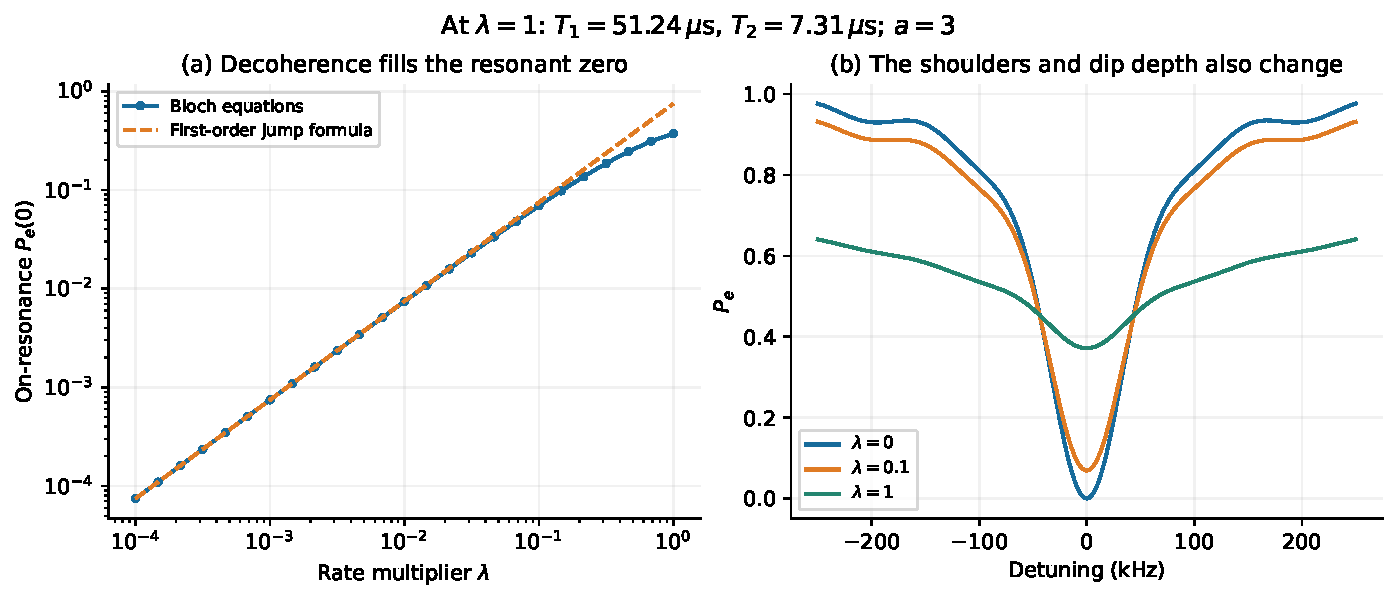
\includegraphics[width=\textwidth]{05_dissipation.pdf}
\caption{Range of validity of the weak-dissipation floor,
Eq.~\eqref{eq:floor}, using $L=20\,\mu$s, $c=0.005$, $a=3$.
Both rates are multiplied by $\lambda$; $\lambda=1$ corresponds to
$T_1=51.24\,\mu$s and $T_2=7.31\,\mu$s. The perturbative result agrees
at small rates but predicts $P_e(0)=0.747$ at $\lambda=1$, whereas full
Bloch evolution gives 0.372. The right panel shows that the shoulders and
dip depth change along with the floor. Adding a constant offset to the
coherent Lorentzian is therefore insufficient. These are two-level model
checks at specified rates, not a fit to experimental data.}
\label{fig:dissipation}
\end{figure}

\section{Numerical checks and use in the manuscript}
We integrate the ideal two-level Schr\"odinger equation with DOP853 in
the coordinate $u=\operatorname{asinh}(t/\tau)$, split at the phase inversion.
The original four-case checker is
\nolinkurl{scripts/check_echo_dip_theory.py}.
For $L=20\,\mu\mathrm{s}$ and $c=0.005$ it gives:
\begin{center}
\begin{tabular}{rrrr}
\toprule
$a$ & $f_{\rm Rabi}$ (MHz) & $2c f_{\rm Rabi}$ (kHz)
 & numerical half-height width (kHz)\\
\midrule
0.3 & 0.955 & 9.55 & no crossing in checked interval\\
1 & 3.183 & 31.83 & 51.41\\
3 & 9.549 & 95.49 & 94.51\\
10 & 31.831 & 318.31 & 320.40\\
\bottomrule
\end{tabular}
\end{center}
The numerical column uses twice the first positive $\Pe=0.5$ crossing;
it is a dip FWHM relative to a unit shoulder only when that shoulder exists.
The checked interval is $0\le\Delta/(\Om_0c)\le4$.
For $a=3,10$, deviations from the simple width are respectively $-1.03\%$
and $+0.66\%$; $a=1$ demonstrates failure outside the strong-drive regime.
Closed-form curvature agrees with direct integration to relative error below
$2\times10^{-6}$ in these checks; tightening solver tolerances changes
sampled populations by less than $1.1\times10^{-9}$.
The square-echo expression also agrees with exact matrix exponentials.
For the weak-dissipation floor, a separate resonant Bloch-equation check
at $a=1.3$, $c=0.05$, and small rates verifies the predicted linear term:
halving both rates reduces the remainder by a factor of $3.999$, as
expected for a second-order error. Arrays, a comparison plot, and exact
parameters are saved under \nolinkurl{outputs/echo_dip_theory/}.
The expanded audit uses \nolinkurl{scripts/plot_echo_dip_theory.py}
and the separate ideal solver \nolinkurl{echospec/simulation/echo_theory.py}.
It tests the full-versus-half propagator identity, Eq.~\eqref{eq:half-identity},
to population error below $1.6\times10^{-9}$ in the sampled root-pulse
checks, and tests the identity for smoothed and polynomial pulses too.
Closed-form $S$ agrees with rotation quadrature within
$6.3\times10^{-10}\,\mu$s. The generalized curvature integral predicts
the near-center populations of all three modified pulses to relative error
below $1.1\times10^{-8}$ at the tested small detuning and 100 MHz.

For the three 100 MHz shaping spectra, halving the detuning-grid spacing
from 0.5 to 0.25 kHz and tightening solver tolerances changes the extracted
window-background widths by less than $4\times10^{-6}$ relatively.
All six focused regression tests pass. The five figures, their underlying
arrays, and source hashes are stored together under
\texttt{figures/paper/echo\_dip\_theory/}; detailed width tables are in
\texttt{outputs/echo\_dip\_theory/}. No experimental acquisitions are
used or modified. The plotted tests do not establish a multilevel or
hardware linewidth, nor a universal strong-dissipation linewidth law.

A suitable central theoretical statement is:
\begin{quote}
The echo symmetry pins an ideal two-level excitation zero to resonance,
whereas the linewidth is governed by how detuning breaks the cancellation.
For a strongly driven root-Lorentzian truncated at a nonzero endpoint
amplitude, adiabatic evolution within the pulse halves yields a Lorentzian
depletion with $\Gamma_f\simeq2c f_{\rm Rabi}$. Removing the endpoint
discontinuity eliminates this particular linear broadening mechanism,
but leaves finite-time nonadiabatic dynamics and dissipation to set the width.
\end{quote}

\section{Comparison with published theory}
Mihov and Vitanov's ordinary-pulse cutoff calculation, Eq.~(3) of
Ref.~\cite{cutoff2024}, contains the Lorentzian factor
$\Om_c^2/(\Om_c^2+\Delta^2)$ multiplying the untruncated pulse's return
probability. It establishes $\Om_c$ as a cutoff-broadening scale.
Our echo calculation produces the complementary central depletion factor
through cancellation of the half-pulse phases. Thus the common endpoint
scale is consistent with that theory, while the echo-specific expression
must be derived from its own propagator, as done here.
All widths here are explicitly full widths, with angular-to-cyclic
conversion $\Gamma_f=\Gamma_\omega/(2\pi)$.

The infinite-wing power-narrowing result in Ref.~\cite{cutoff2024}
requires a decay exponent larger than one. The root-Lorentzian is its
marginal boundary, so substituting $n=1/2$ into that scaling cannot yield
its finite-pulse FWHM.

For ordinary finite-duration pulses, Ref.~\cite{edges2013} gives the
large-drive scale $\Om_0^{1/(m+1)}$ when the first discontinuous endpoint
derivative has order $m$. Our polynomial envelope starts as $s^{p+1}$,
so $m=p+1$ and the candidate exponent is $1/(p+2)$. This supports the
edge dimensional argument, not an exact echo spectrum or its numerical
prefactor. Ref.~\cite{smooth2024} likewise separates nonadiabatic edges
from an adiabatic interior for pulses with linear edges; its explicit
line-shape formulas do not directly describe a sixth-order edge.

\begin{thebibliography}{9}
\bibitem{rotary1980} N. C. Wong, S. S. Kano, and R. G. Brewer,
Optical rotary echoes, \emph{Phys. Rev. A} \textbf{21}, 260 (1980).
\href{https://doi.org/10.1103/PhysRevA.21.260}{doi:10.1103/PhysRevA.21.260}.
\bibitem{cutoff2024} I. S. Mihov and N. V. Vitanov,
Defying Conventional Wisdom in Spectroscopy: Power Narrowing on IBM Quantum,
\emph{Phys. Rev. Lett.} \textbf{132}, 020802 (2024).
\href{https://arxiv.org/abs/2308.14187}{arXiv:2308.14187}.
\bibitem{edges2013} I. I. Boradjiev and N. V. Vitanov,
Control of qubits by shaped pulses of finite duration,
\emph{Phys. Rev. A} \textbf{88}, 013402 (2013).
\href{https://doi.org/10.1103/PhysRevA.88.013402}{doi:10.1103/PhysRevA.88.013402}.
\bibitem{smooth2024} I. S. Mihov and N. V. Vitanov,
Qubit dynamics driven by smooth pulses of finite duration,
\emph{Phys. Rev. A} \textbf{110}, 052609 (2024).
\href{https://arxiv.org/abs/2404.12236}{arXiv:2404.12236}.
\end{thebibliography}
\end{document}
